%%____________________________________________________________________________||
\section{Data sets and simulation}
\label{app:datasets}

\begin{table}[h!]
  \topcaption{List of primary data sets used in this analysis.}
  \footnotesize 
  \begin{center}
\begin{tabular}{l}
\hline\hline
\multicolumn{1}{c}{Data set}\tabularnewline
\hline
\verb!/HTMHT/Run2016B-23Sep2016-v3/MINIAOD!\tabularnewline
\verb!/HTMHT/Run2016C-23Sep2016-v1/MINIAOD!\tabularnewline
\verb!/HTMHT/Run2016D-23Sep2016-v1/MINIAOD!\tabularnewline
\verb!/HTMHT/Run2016E-23Sep2016-v1/MINIAOD!\tabularnewline
\verb!/HTMHT/Run2016F-23Sep2016-v1/MINIAOD!\tabularnewline
\verb!/HTMHT/Run2016G-23Sep2016-v2/MINIAOD!\tabularnewline
\verb!/HTMHT/Run2016H-PromptReco-v2/MINIAOD!\tabularnewline
\verb!/HTMHT/Run2016H-PromptReco-v3/MINIAOD!\tabularnewline
\verb!/JetHT/Run2016B-23Sep2016-v2/MINIAOD!\tabularnewline
\verb!/JetHT/Run2016C-23Sep2016-v2/MINIAOD!\tabularnewline
\verb!/JetHT/Run2016D-23Sep2016-v2/MINIAOD!\tabularnewline
\verb!/JetHT/Run2016E-23Sep2016-v1/MINIAOD!\tabularnewline
\verb!/JetHT/Run2016F-23Sep2016-v1/MINIAOD!\tabularnewline
\verb!/JetHT/Run2016G-23Sep2016-v2/MINIAOD!\tabularnewline
\verb!/JetHT/Run2016H-PromptReco-v2/MINIAOD!\tabularnewline
\verb!/JetHT/Run2016H-PromptReco-v3/MINIAOD!\tabularnewline
\verb!/MET/Run2016B-23Sep2016-v3/MINIAOD!\tabularnewline
\verb!/MET/Run2016C-23Sep2016-v1/MINIAOD!\tabularnewline
\verb!/MET/Run2016D-23Sep2016-v1/MINIAOD!\tabularnewline
\verb!/MET/Run2016E-23Sep2016-v1/MINIAOD!\tabularnewline
\verb!/MET/Run2016F-23Sep2016-v1/MINIAOD!\tabularnewline
\verb!/MET/Run2016G-23Sep2016-v1/MINIAOD!\tabularnewline
\verb!/MET/Run2016H-PromptReco-v2/MINIAOD!\tabularnewline
\verb!/SingleMuon/Run2016B-23Sep2016-v3/MINIAOD!\tabularnewline
\verb!/SingleMuon/Run2016C-23Sep2016-v1/MINIAOD!\tabularnewline
\verb!/SingleMuon/Run2016D-23Sep2016-v1/MINIAOD!\tabularnewline
\verb!/SingleMuon/Run2016E-23Sep2016-v1/MINIAOD!\tabularnewline
\verb!/SingleMuon/Run2016F-23Sep2016-v1/MINIAOD!\tabularnewline
\verb!/SingleMuon/Run2016G-23Sep2016-v1/MINIAOD!\tabularnewline
\verb!/SingleMuon/Run2016H-PromptReco-v2/MINIAOD!\tabularnewline
\verb!/SingleMuon/Run2016H-PromptReco-v3/MINIAOD!\tabularnewline
\verb!/SinglePhoton/Run2016B-23Sep2016-v3/MINIAOD!\tabularnewline
\verb!/SinglePhoton/Run2016C-23Sep2016-v1/MINIAOD!\tabularnewline
\verb!/SinglePhoton/Run2016D-23Sep2016-v1/MINIAOD!\tabularnewline
\verb!/SinglePhoton/Run2016E-23Sep2016-v1/MINIAOD!\tabularnewline
\verb!/SinglePhoton/Run2016F-23Sep2016-v1/MINIAOD!\tabularnewline
\verb!/SinglePhoton/Run2016G-23Sep2016-v1/MINIAOD!\tabularnewline
\verb!/SinglePhoton/Run2016H-PromptReco-v2/MINIAOD!\tabularnewline
\verb!/SinglePhoton/Run2016H-PromptReco-v3/MINIAOD!\tabularnewline
\verb!/DoubleEG/Run2016B-23Sep2016-v3/MINIAOD!\tabularnewline
\verb!/DoubleEG/Run2016C-23Sep2016-v1/MINIAOD!\tabularnewline
\verb!/DoubleEG/Run2016D-23Sep2016-v1/MINIAOD!\tabularnewline
\verb!/DoubleEG/Run2016E-23Sep2016-v1/MINIAOD!\tabularnewline
\verb!/DoubleEG/Run2016F-23Sep2016-v1/MINIAOD!\tabularnewline
\verb!/DoubleEG/Run2016G-23Sep2016-v1/MINIAOD!\tabularnewline
\verb!/DoubleEG/Run2016H-PromptReco-v2/MINIAOD!\tabularnewline
\verb!/DoubleEG/Run2016H-PromptReco-v3/MINIAOD!\tabularnewline
\hline
\end{tabular}\end{center}

  \label{tab:datasets_data}
\end{table}

\begin{table}[h!]
  \centering
  \topcaption{Simulated event samples of SM background processes used
    by this analysis. Symbols used as shorthand are defined at the
    bottom of the table.
    Other samples are described in Table~\ref{tab:datasets_bkg2}}
  \fontsize{7}{8.4}\selectfont
  %latex.default(d, title = NULL, booktabs = FALSE, width = 3, rowname = NULL,     helvetica = FALSE, caption.loc = "bottom", ...)%
\begin{center}
\begin{tabular}{ll}
\hline\hline
\multicolumn{1}{c}{Data set}&\multicolumn{1}{c}{Cross section [pb]}\tabularnewline
\hline
\verb!/ZJetsToNuNu_HT-100To200_13TeV-madgraph/[1]-v1/MINIAODSIM! &$3.448\times 10^{+02}$\tabularnewline
\verb!/ZJetsToNuNu_HT-100To200_13TeV-madgraph/[1]_ext1-v1/MINIAODSIM! &$3.448\times 10^{+02}$\tabularnewline
\verb!/ZJetsToNuNu_HT-200To400_13TeV-madgraph/[1]-v1/MINIAODSIM! &$9.553\times 10^{+01}$\tabularnewline
\verb!/ZJetsToNuNu_HT-200To400_13TeV-madgraph/[1]_ext1-v1/MINIAODSIM! &$9.553\times 10^{+01}$\tabularnewline
\verb!/ZJetsToNuNu_HT-400To600_13TeV-madgraph/[1]-v1/MINIAODSIM! &$1.320\times 10^{+01}$\tabularnewline
\verb!/ZJetsToNuNu_HT-400To600_13TeV-madgraph/[1]_ext1-v1/MINIAODSIM! &$1.320\times 10^{+01}$\tabularnewline
\verb!/ZJetsToNuNu_HT-600To800_13TeV-madgraph/[1]-v1/MINIAODSIM! &$3.221\times 10^{+00}$\tabularnewline
\verb!/ZJetsToNuNu_HT-800To1200_13TeV-madgraph/[1]-v1/MINIAODSIM! &$1.474\times 10^{+00}$\tabularnewline
\verb!/ZJetsToNuNu_HT-1200To2500_13TeV-madgraph/[1]-v1/MINIAODSIM! &$3.586\times 10^{-01}$\tabularnewline
\verb!/ZJetsToNuNu_HT-1200To2500_13TeV-madgraph/[1]_ext1-v1/MINIAODSIM! &$3.586\times 10^{-01}$\tabularnewline
\verb!/ZJetsToNuNu_HT-2500ToInf_13TeV-madgraph/[1]-v1/MINIAODSIM! &$8.203\times 10^{-03}$\tabularnewline
\verb!/WJetsToLNu_HT-100To200_[2]/[1]-v1/MINIAODSIM! &$1.627\times 10^{+03}$\tabularnewline
\verb!/WJetsToLNu_HT-100To200_[2]/[1]_ext1-v1/MINIAODSIM! &$1.627\times 10^{+03}$\tabularnewline
\verb!/WJetsToLNu_HT-100To200_[2]/[1]_ext2-v1/MINIAODSIM! &$1.627\times 10^{+03}$\tabularnewline
\verb!/WJetsToLNu_HT-200To400_[2]/[1]-v1/MINIAODSIM! &$4.352\times 10^{+02}$\tabularnewline
\verb!/WJetsToLNu_HT-200To400_[2]/[1]_ext1-v1/MINIAODSIM! &$4.352\times 10^{+02}$\tabularnewline
\verb!/WJetsToLNu_HT-200To400_[2]/[1]_ext2-v1/MINIAODSIM! &$4.352\times 10^{+02}$\tabularnewline
\verb!/WJetsToLNu_HT-400To600_[2]/[1]-v1/MINIAODSIM! &$5.918\times 10^{+01}$\tabularnewline
\verb!/WJetsToLNu_HT-400To600_[2]/[1]_ext1-v1/MINIAODSIM! &$5.918\times 10^{+01}$\tabularnewline
\verb!/WJetsToLNu_HT-600To800_[2]/[1]-v1/MINIAODSIM! &$1.458\times 10^{+01}$\tabularnewline
\verb!/WJetsToLNu_HT-600To800_[2]/[1]_ext1-v1/MINIAODSIM! &$1.458\times 10^{+01}$\tabularnewline
\verb!/WJetsToLNu_HT-800To1200_[2]/[1]-v1/MINIAODSIM! &$6.656\times 10^{+00}$\tabularnewline
\verb!/WJetsToLNu_HT-800To1200_[2]/[1]_ext1-v1/MINIAODSIM! &$6.656\times 10^{+00}$\tabularnewline
\verb!/WJetsToLNu_HT-1200To2500_[2]/[1]-v1/MINIAODSIM! &$1.608\times 10^{+00}$\tabularnewline
\verb!/WJetsToLNu_HT-1200To2500_[2]/[1]_ext1-v1/MINIAODSIM! &$1.608\times 10^{+00}$\tabularnewline
\verb!/WJetsToLNu_HT-2500ToInf_[2]/[1]-v1/MINIAODSIM! &$3.891\times 10^{-02}$\tabularnewline
\verb!/WJetsToLNu_HT-2500ToInf_[2]/[1]_ext1-v1/MINIAODSIM! &$3.891\times 10^{-02}$\tabularnewline
\verb!/TTJets_DiLept_[2]/[1]-v1/MINIAODSIM! &$8.829\times 10^{+01}$\tabularnewline
\verb!/TTJets_DiLept_[2]/[1]_ext1-v1/MINIAODSIM! &$8.829\times 10^{+01}$\tabularnewline
\verb!/TTJets_HT-600to800_[2]/[1]_ext1-v1/MINIAODSIM! &$2.734\times 10^{+00}$\tabularnewline
\verb!/TTJets_HT-800to1200_[2]/[1]_ext1-v1/MINIAODSIM! &$1.121\times 10^{+00}$\tabularnewline
\verb!/TTJets_HT-1200to2500_[2]/[1]_ext1-v1/MINIAODSIM! &$1.979\times 10^{-01}$\tabularnewline
\verb!/TTJets_HT-2500toInf_[2]/[1]_ext1-v1/MINIAODSIM! &$2.368\times 10^{-03}$\tabularnewline
\verb!/TTJets_SingleLeptFromT_[2]/[1]-v1/MINIAODSIM! &$1.827\times 10^{+02}$\tabularnewline
\verb!/TTJets_SingleLeptFromT_[2]/[1]_ext1-v1/MINIAODSIM! &$1.827\times 10^{+02}$\tabularnewline
\verb!/TTJets_SingleLeptFromTbar_[2]/[1]-v1/MINIAODSIM! &$1.827\times 10^{+02}$\tabularnewline
\verb!/TTJets_SingleLeptFromTbar_[2]/[1]_ext1-v1/MINIAODSIM! &$1.827\times 10^{+02}$\tabularnewline
\verb!/DYJetsToLL_M-50_HT-100to200_[2]/[1]-v1/MINIAODSIM! &$1.813\times 10^{+02}$\tabularnewline
\verb!/DYJetsToLL_M-50_HT-100to200_[2]/[1]_ext1-v1/MINIAODSIM! &$1.813\times 10^{+02}$\tabularnewline
\verb!/DYJetsToLL_M-50_HT-200to400_[2]/[1]-v1/MINIAODSIM! &$5.042\times 10^{+01}$\tabularnewline
\verb!/DYJetsToLL_M-50_HT-200to400_[2]/[1]_ext1-v1/MINIAODSIM! &$5.042\times 10^{+01}$\tabularnewline
\verb!/DYJetsToLL_M-50_HT-400to600_[2]/[1]-v1/MINIAODSIM! &$6.984\times 10^{+00}$\tabularnewline
\verb!/DYJetsToLL_M-50_HT-400to600_[2]/[1]_ext1-v1/MINIAODSIM! &$6.984\times 10^{+00}$\tabularnewline
\verb!/DYJetsToLL_M-50_HT-600to800_[2]/[1]-v2/MINIAODSIM! &$1.681\times 10^{+00}$\tabularnewline
\verb!/DYJetsToLL_M-50_HT-800to1200_[2]/[1]-v1/MINIAODSIM! &$7.754\times 10^{-01}$\tabularnewline
\verb!/DYJetsToLL_M-50_HT-1200to2500_[2]/[1]-v1/MINIAODSIM! &$1.862\times 10^{-01}$\tabularnewline
\verb!/DYJetsToLL_M-50_HT-2500toInf_[2]/[1]-v1/MINIAODSIM! &$4.385\times 10^{-03}$\tabularnewline
\verb!/GJets_HT-40To100_[2]/[1]-v1/MINIAODSIM! &$2.079\times 10^{+04}$\tabularnewline
\verb!/GJets_HT-40To100_[2]/[1]_ext1-v1/MINIAODSIM! &$2.079\times 10^{+04}$\tabularnewline
\verb!/GJets_HT-100To200_[2]/[1]-v1/MINIAODSIM! &$9.238\times 10^{+03}$\tabularnewline
\verb!/GJets_HT-100To200_[2]/[1]_ext1-v1/MINIAODSIM! &$9.238\times 10^{+03}$\tabularnewline
\verb!/GJets_HT-200To400_[2]/[1]-v1/MINIAODSIM! &$2.305\times 10^{+03}$\tabularnewline
\verb!/GJets_HT-200To400_[2]/[1]_ext1-v1/MINIAODSIM! &$2.305\times 10^{+03}$\tabularnewline
\verb!/GJets_HT-400To600_[2]/[1]-v1/MINIAODSIM! &$2.744\times 10^{+02}$\tabularnewline
\verb!/GJets_HT-400To600_[2]/[1]_ext1-v2/MINIAODSIM! &$2.744\times 10^{+02}$\tabularnewline
\verb!/GJets_HT-600ToInf_[2]/[1]-v1/MINIAODSIM! &$9.346\times 10^{+01}$\tabularnewline
\verb!/GJets_HT-600ToInf_[2]/[1]_ext1-v1/MINIAODSIM! &$9.346\times 10^{+01}$\tabularnewline
\hline
\multicolumn{1}{l}{String} & \multicolumn{1}{l}{Symbol} \tabularnewline
\verb!RunIISummer16MiniAODv2-PUMoriond17_80X_mcRun2_asymptotic_2016_TrancheIV_v6! & \verb![1]! \tabularnewline
\verb!TuneCUETP8M1_13TeV-madgraphMLM-pythia8! & \verb![2]! \tabularnewline
\hline
\hline
\end{tabular}\end{center}

  \label{tab:datasets_bkg}
\end{table}

\begin{table}[h!]
  \centering
  \topcaption{Simulated event samples of SM background processes used
    by this analysis. Symbols used as shorthand are defined at the
    bottom of the table.
    Other samples are described in Table~\ref{tab:datasets_bkg}}
  \fontsize{7}{8.4}\selectfont
  %latex.default(d, title = NULL, booktabs = FALSE, width = 3, rowname = NULL,     helvetica = FALSE, caption.loc = "bottom", ...)%
\begin{center}
\begin{tabular}{ll}
\hline\hline
\multicolumn{1}{c}{Data set}&\multicolumn{1}{c}{Cross section [pb]}\tabularnewline
\hline
\verb!/QCD_HT100to200_[2]/[1]-v1/MINIAODSIM! &$2.799\times 10^{+07}$\tabularnewline
\verb!/QCD_HT200to300_[2]/[1]-v1/MINIAODSIM! &$1.712\times 10^{+06}$\tabularnewline
\verb!/QCD_HT200to300_[2]/[1]_ext1-v1/MINIAODSIM! &$1.712\times 10^{+06}$\tabularnewline
\verb!/QCD_HT300to500_[2]/[1]-v1/MINIAODSIM! &$3.477\times 10^{+05}$\tabularnewline
\verb!/QCD_HT300to500_[2]/[1]_ext1-v1/MINIAODSIM! &$3.477\times 10^{+05}$\tabularnewline
\verb!/QCD_HT500to700_[2]/[1]-v1/MINIAODSIM! &$3.210\times 10^{+04}$\tabularnewline
\verb!/QCD_HT500to700_[2]/[1]_ext1-v2/MINIAODSIM! &$3.210\times 10^{+04}$\tabularnewline
\verb!/QCD_HT700to1000_[2]/[1]-v1/MINIAODSIM! &$6.831\times 10^{+03}$\tabularnewline
\verb!/QCD_HT700to1000_[2]/[1]_ext1-v1/MINIAODSIM! &$6.831\times 10^{+03}$\tabularnewline
\verb!/QCD_HT1000to1500_[2]/[1]-v1/MINIAODSIM! &$1.207\times 10^{+03}$\tabularnewline
\verb!/QCD_HT1000to1500_[2]/[1]_ext1-v1/MINIAODSIM! &$1.207\times 10^{+03}$\tabularnewline
\verb!/QCD_HT1500to2000_[2]/[1]-v1/MINIAODSIM! &$1.199\times 10^{+02}$\tabularnewline
\verb!/QCD_HT1500to2000_[2]/[1]_ext1-v1/MINIAODSIM! &$1.199\times 10^{+02}$\tabularnewline
\verb!/QCD_HT2000toInf_[2]/[1]-v1/MINIAODSIM! &$2.524\times 10^{+01}$\tabularnewline
\verb!/QCD_HT2000toInf_[2]/[1]_ext1-v1/MINIAODSIM! &$2.524\times 10^{+01}$\tabularnewline
\verb!/ST_s-channel_4f_leptonDecays_[3]/[1]-v1/MINIAODSIM! &$3.344\times 10^{+00}$\tabularnewline
\verb!/ST_tW_antitop_5f_inclusiveDecays_[4]/[1]_ext1-v1/MINIAODSIM! &$3.560\times 10^{+01}$\tabularnewline
\verb!/ST_tW_top_5f_inclusiveDecays_[4]/[1]_ext1-v1/MINIAODSIM! &$3.560\times 10^{+01}$\tabularnewline
\verb!/ST_t-channel_antitop_4f_inclusiveDecays_[5]/[1]-v1/MINIAODSIM! &$8.095\times 10^{+01}$\tabularnewline
\verb!/ST_t-channel_top_4f_inclusiveDecays_[5]/[1]-v1/MINIAODSIM! &$1.360\times 10^{+02}$\tabularnewline
\verb!/TTWJetsToLNu_[6]FXFX-madspin-pythia8/[1]_ext1-v3/MINIAODSIM! &$2.043\times 10^{-01}$\tabularnewline
\verb!/TTWJetsToLNu_[6]FXFX-madspin-pythia8/[1]_ext2-v1/MINIAODSIM! &$2.043\times 10^{-01}$\tabularnewline
\verb!/TTWJetsToQQ_[6]FXFX-madspin-pythia8/[1]-v1/MINIAODSIM! &$4.062\times 10^{-01}$\tabularnewline
\verb!/TTZToLLNuNu_M-10_[6]-pythia8/[1]_ext1-v1/MINIAODSIM! &$2.529\times 10^{-01}$\tabularnewline
\verb!/TTZToQQ_[6]-pythia8/[1]-v1/MINIAODSIM! &$5.297\times 10^{-01}$\tabularnewline
\verb!/TTGJets_[6]FXFX-madspin-pythia8/[1]-v1/MINIAODSIM! &$3.697\times 10^{+00}$\tabularnewline
\verb!/TTGJets_[6]FXFX-madspin-pythia8/[1]_ext1-v1/MINIAODSIM! &$3.697\times 10^{+00}$\tabularnewline
\verb!/ttHToNonbb_M125_TuneCUETP8M2_ttHtranche3_[7]/[1]-v1/MINIAODSIM! &$2.151\times 10^{-01}$\tabularnewline
\verb!/ttHTobb_M125_TuneCUETP8M2_ttHtranche3_[7]/[1]-v1/MINIAODSIM! &$2.934\times 10^{-01}$\tabularnewline
\verb!/WW_TuneCUETP8M1_13TeV-pythia8/[1]-v1/MINIAODSIM! &$1.139\times 10^{+02}$\tabularnewline
\verb!/WW_TuneCUETP8M1_13TeV-pythia8/[1]_ext1-v1/MINIAODSIM! &$1.139\times 10^{+02}$\tabularnewline
\verb!/WZ_TuneCUETP8M1_13TeV-pythia8/[1]-v1/MINIAODSIM! &$4.713\times 10^{+01}$\tabularnewline
\verb!/WZ_TuneCUETP8M1_13TeV-pythia8/[1]_ext1-v1/MINIAODSIM! &$4.713\times 10^{+01}$\tabularnewline
\verb!/ZZ_TuneCUETP8M1_13TeV-pythia8/[1]-v1/MINIAODSIM! &$1.652\times 10^{+01}$\tabularnewline
\verb!/ZZ_TuneCUETP8M1_13TeV-pythia8/[1]_ext1-v1/MINIAODSIM! &$1.652\times 10^{+01}$\tabularnewline
\verb!/EWKWMinus2Jets_WToLNu_M-50_13TeV-madgraph-pythia8/[1]-v1/MINIAODSIM! &$1.000\times 10^{+00}$\tabularnewline
\verb!/EWKWPlus2Jets_WToLNu_M-50_13TeV-madgraph-pythia8/[1]-v1/MINIAODSIM! &$1.000\times 10^{+00}$\tabularnewline
\verb!/EWKZ2Jets_ZToLL_M-50_13TeV-madgraph-pythia8/[1]-v1/MINIAODSIM! &$1.000\times 10^{+00}$\tabularnewline
\verb!/EWKZ2Jets_ZToNuNu_13TeV-madgraph-pythia8/[1]-v1/MINIAODSIM! &$1.000\times 10^{+00}$\tabularnewline
\hline
\multicolumn{1}{l}{String} & \multicolumn{1}{l}{Symbol} \tabularnewline
\verb!RunIISummer16MiniAODv2-PUMoriond17_80X_mcRun2_asymptotic_2016_TrancheIV_v6! & \verb![1]! \tabularnewline
\verb!TuneCUETP8M1_13TeV-madgraphMLM-pythia8! & \verb![2]! \tabularnewline
\verb!13TeV-amcatnlo-pythia8_TuneCUETP8M1! & \verb![3]! \tabularnewline
\verb!13TeV-powheg-pythia8_TuneCUETP8M1! & \verb![4]! \tabularnewline
\verb!13TeV-powhegV2-madspin-pythia8_TuneCUETP8M1! & \verb![5]! \tabularnewline
\verb!TuneCUETP8M1_13TeV-amcatnlo! & \verb![6]! \tabularnewline
\verb!TuneCUETP8M2_ttHtranche3_13TeV-powheg-pythia8! & \verb![7]! \tabularnewline
\hline
\hline
\end{tabular}\end{center}

%\verb!/GJets_DR-0p4_HT-40To100_[2]/[2]-v1/MINIAODSIM! &$1.856\times 10^{+04}$\tabularnewline
%\verb!/GJets_DR-0p4_HT-100To200_[2]/[2]-v1/MINIAODSIM! &$5.000\times 10^{+03}$\tabularnewline
%\verb!/GJets_DR-0p4_HT-200To400_[2]/[2]-v1/MINIAODSIM! &$1.079\times 10^{+03}$\tabularnewline
%\verb!/GJets_DR-0p4_HT-400To600_[2]/[2]-v1/MINIAODSIM! &$1.259\times 10^{+02}$\tabularnewline
%\verb!/GJets_DR-0p4_HT-600ToInf_[2]/[2]-v1/MINIAODSIM! &$4.336\times 10^{+01}$\tabularnewline
%RunIISummer16MiniAODv2-PUMoriond17_qcut19_80X_mcRun2_asymptotic_2016_TrancheIV_v6 [1]

  \label{tab:datasets_bkg2}
\end{table}

\begin{figure}[!h]
  \begin{center}
    \subfigure[$Z\rightarrow \nu\nu$ + jets]{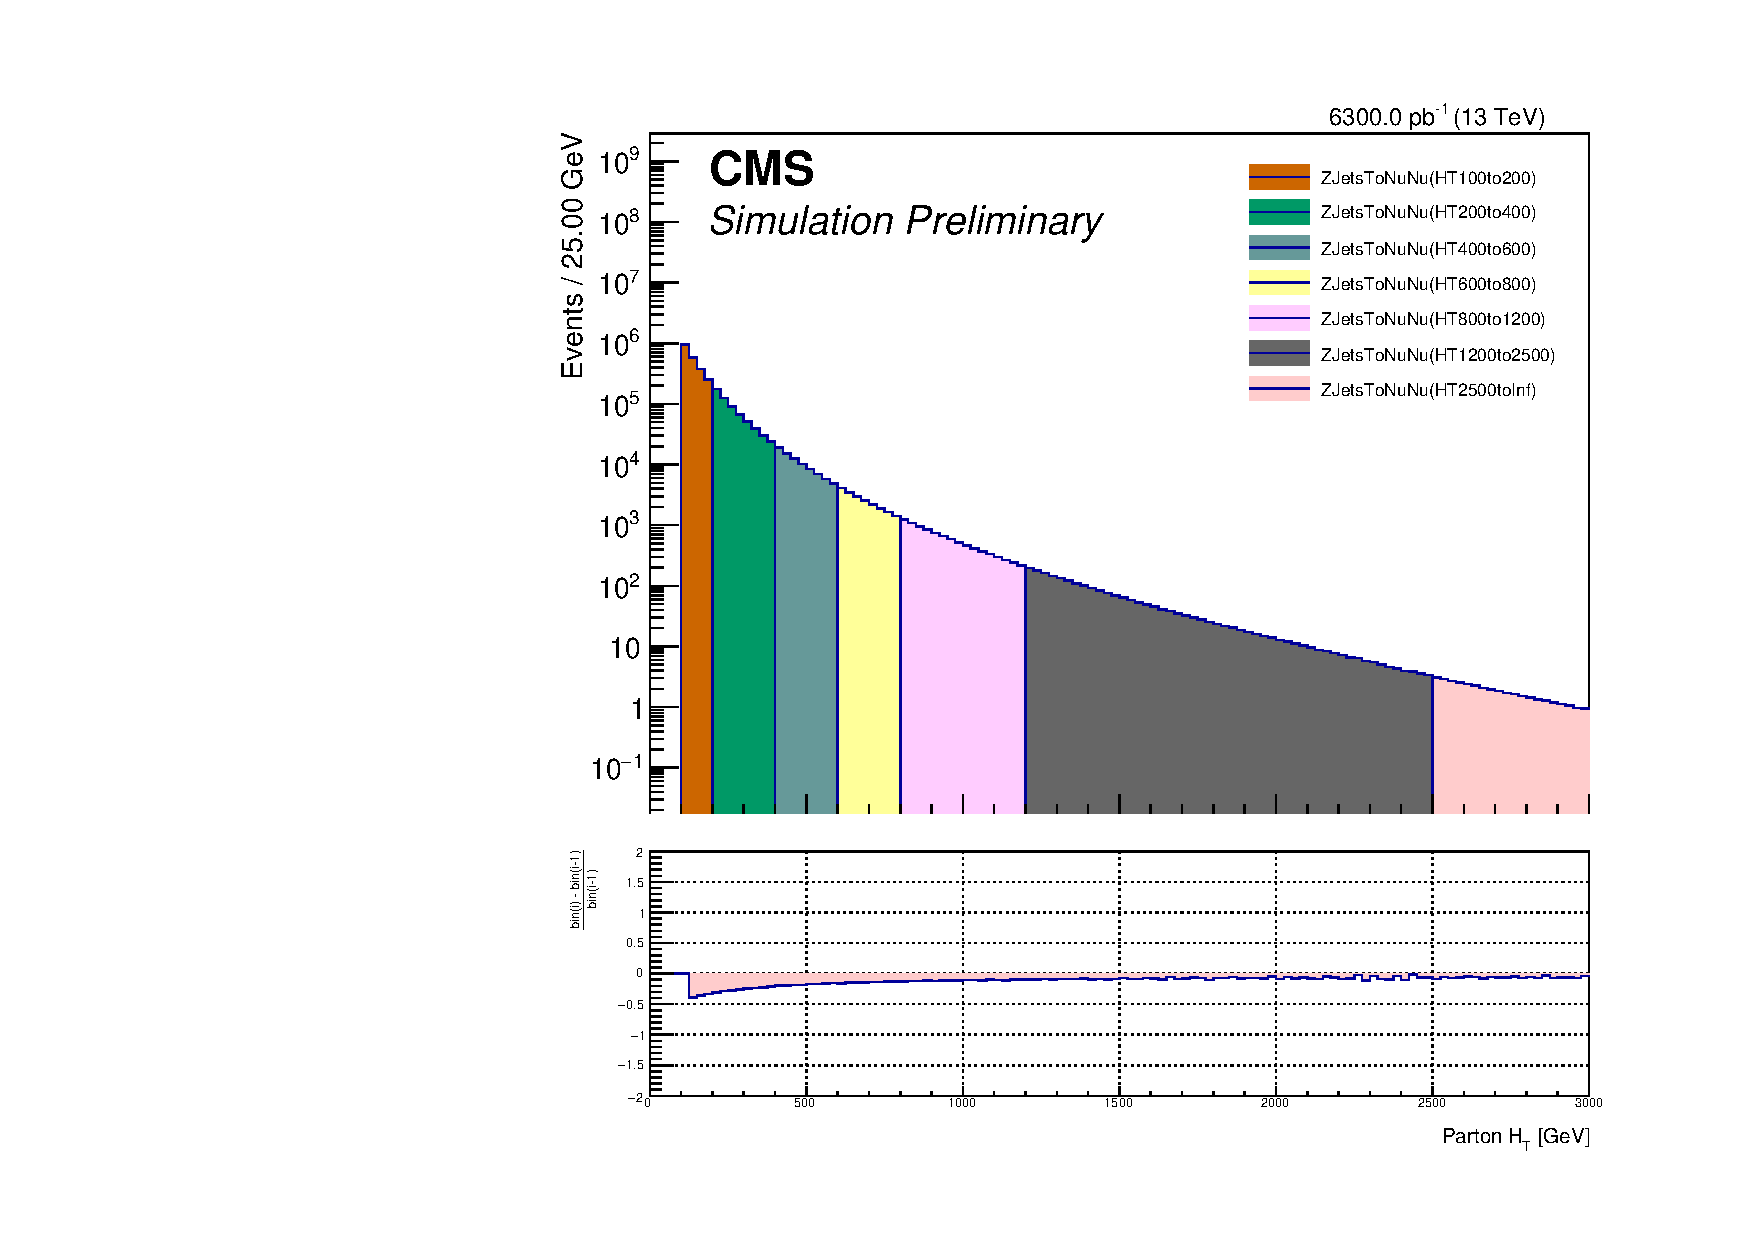
\includegraphics[width=0.35\textwidth]{figures/binnedMCsamples/Zinv.pdf}} ~
    \subfigure[$W\rightarrow l \nu$ + jets]{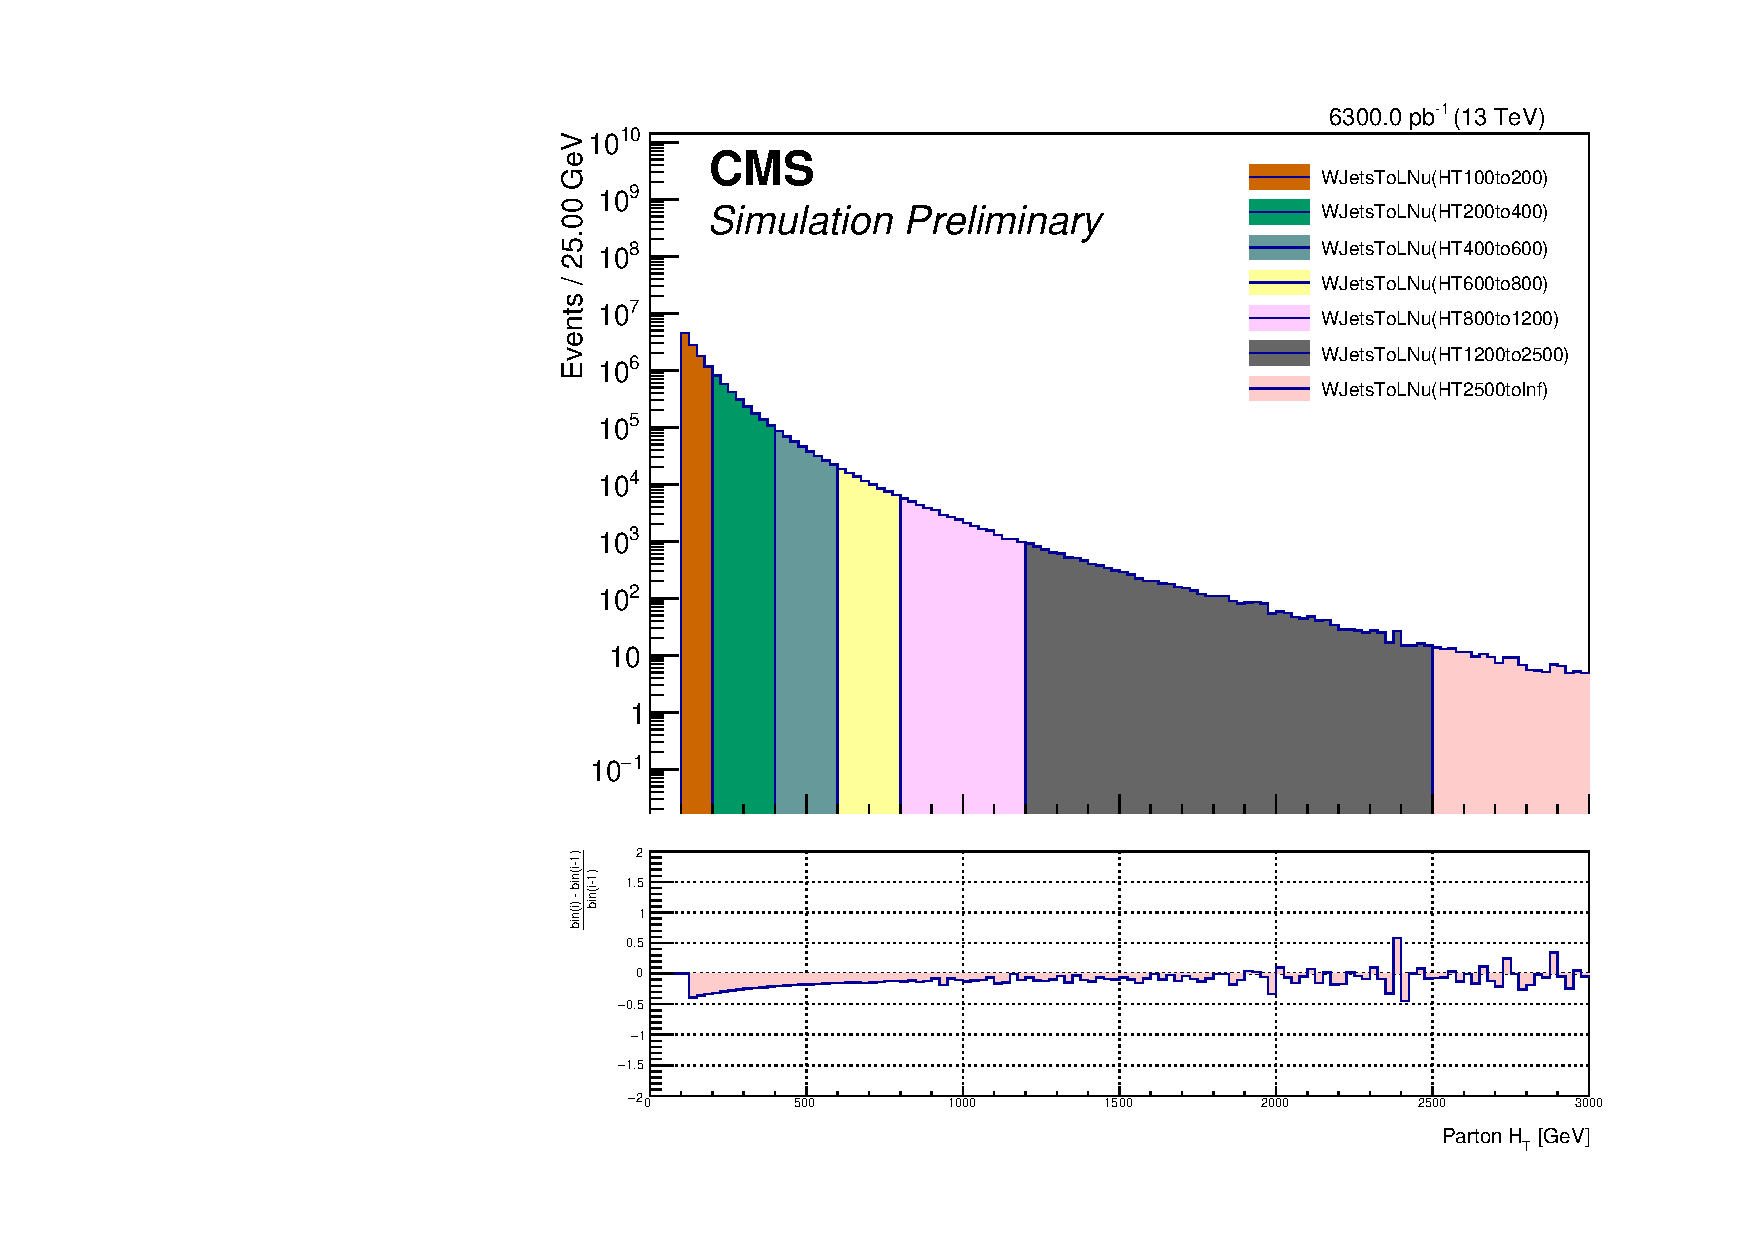
\includegraphics[width=0.35\textwidth]{figures/binnedMCsamples/WJetsToLNu_HT.pdf}} \\
    \subfigure[$DY\rightarrow ll$ + jets]{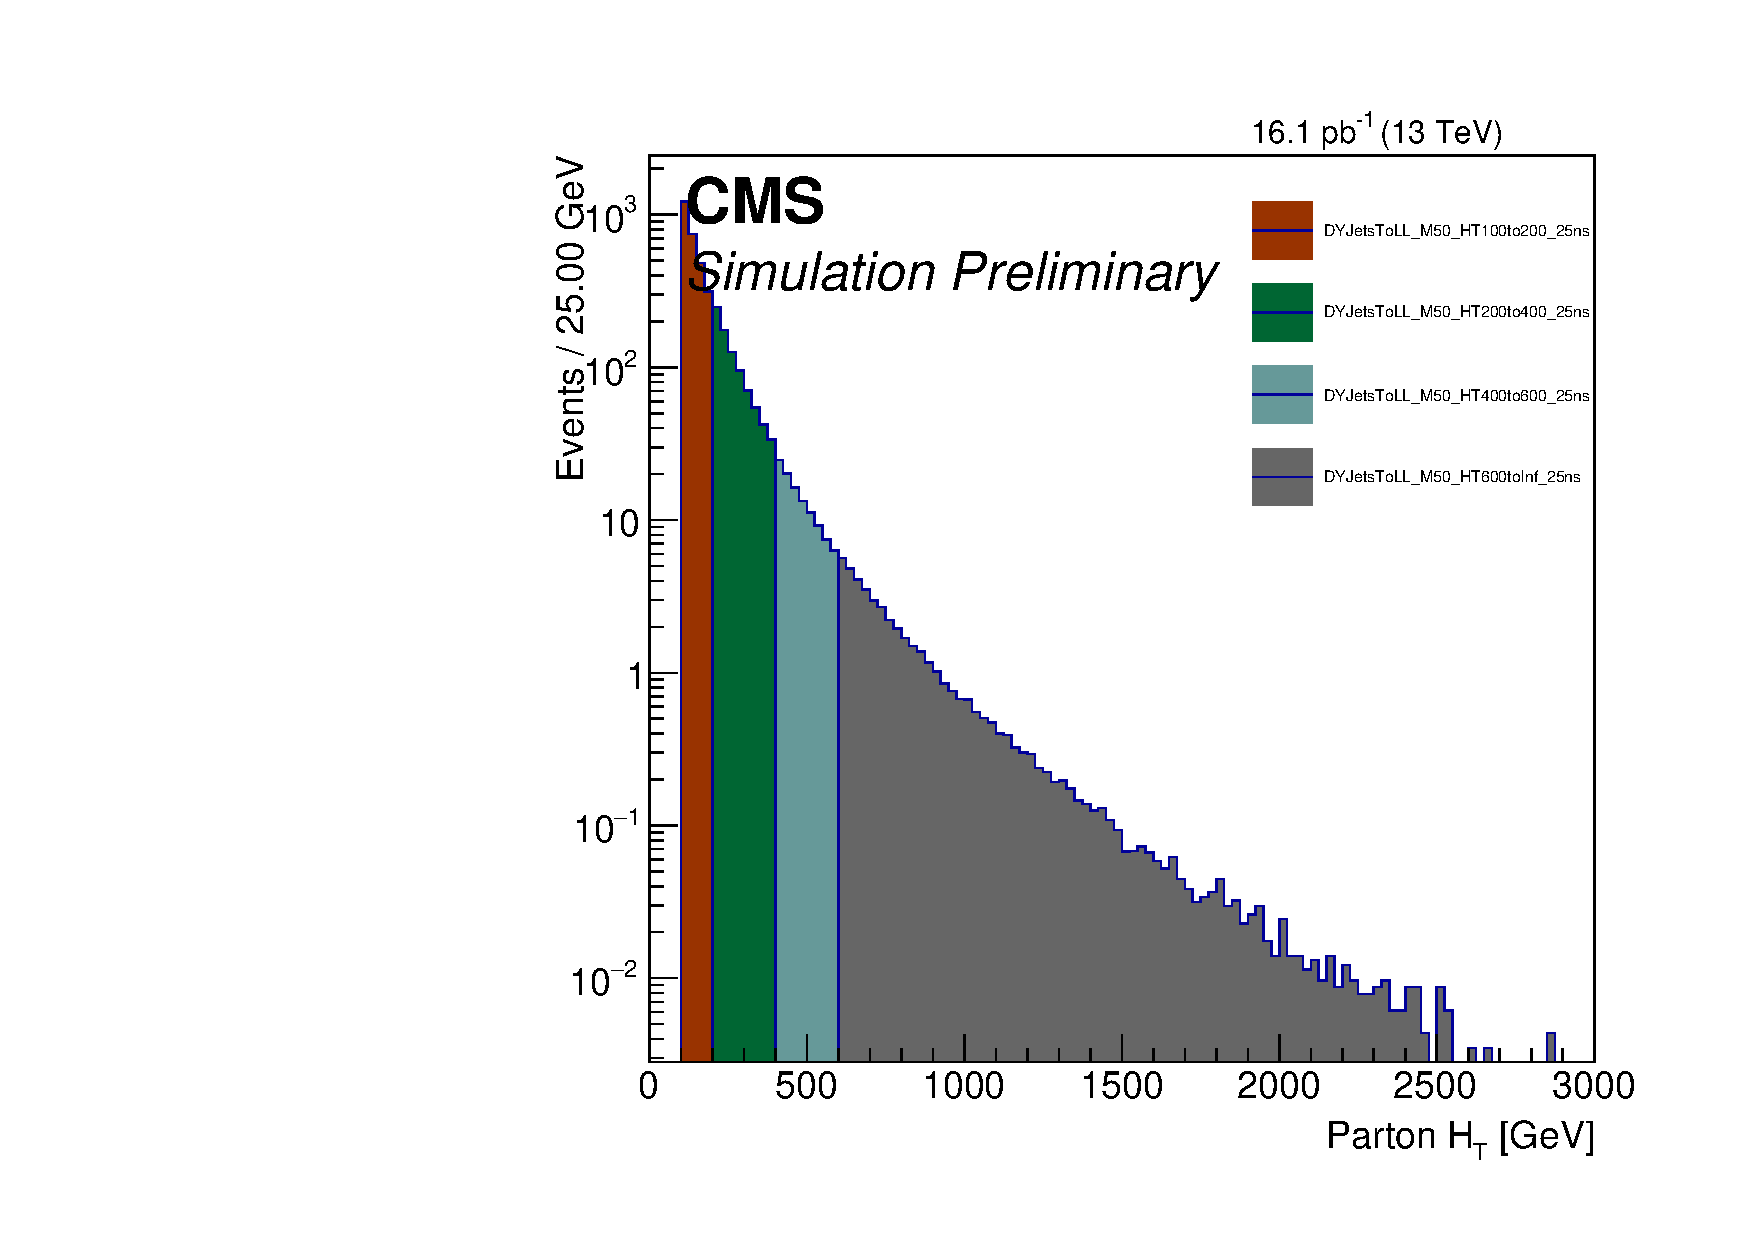
\includegraphics[width=0.35\textwidth]{figures/binnedMCsamples/DYJetsToLL_M50_HT.pdf}} ~
    \subfigure[QCD]{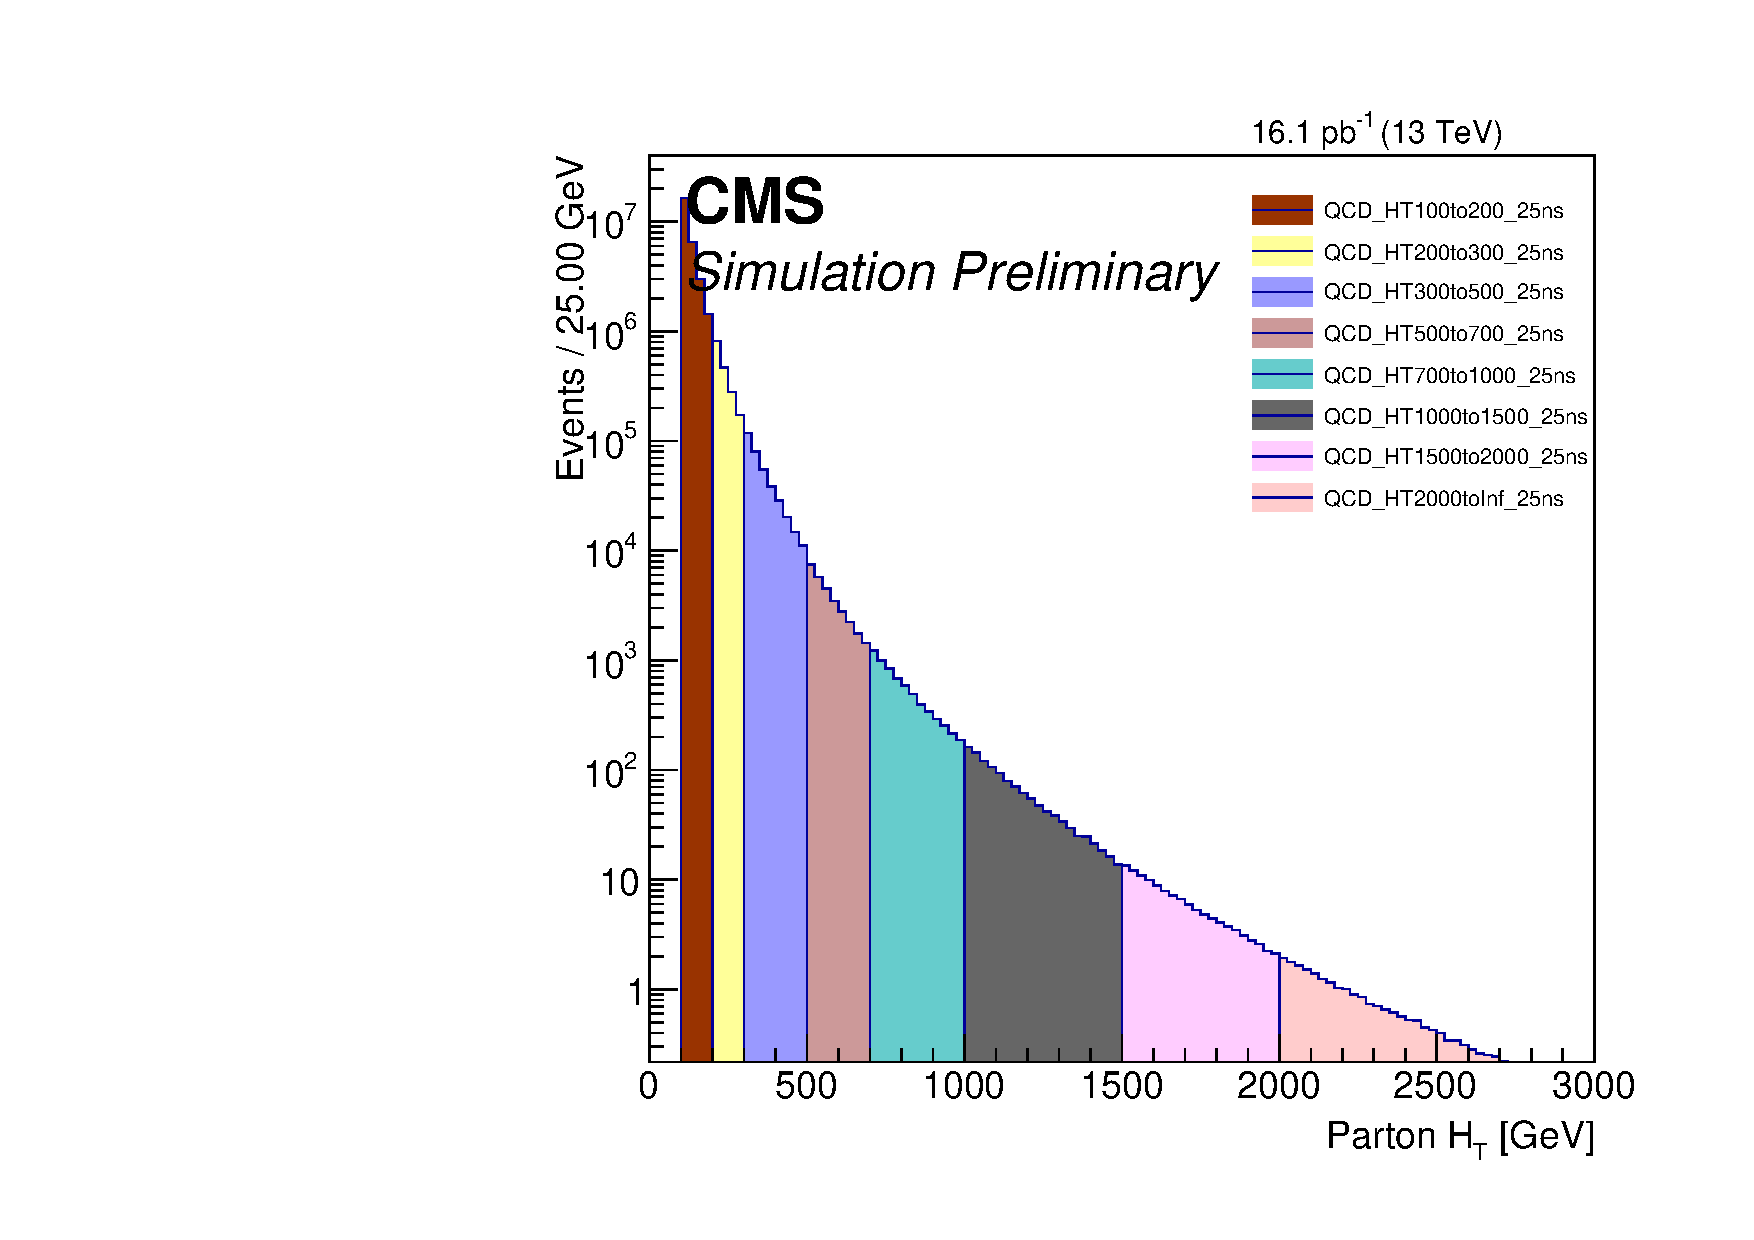
\includegraphics[width=0.40\textwidth]{figures/binnedMCsamples/QCD_HT.pdf}} \\
    \subfigure[$\gamma$ + jets]{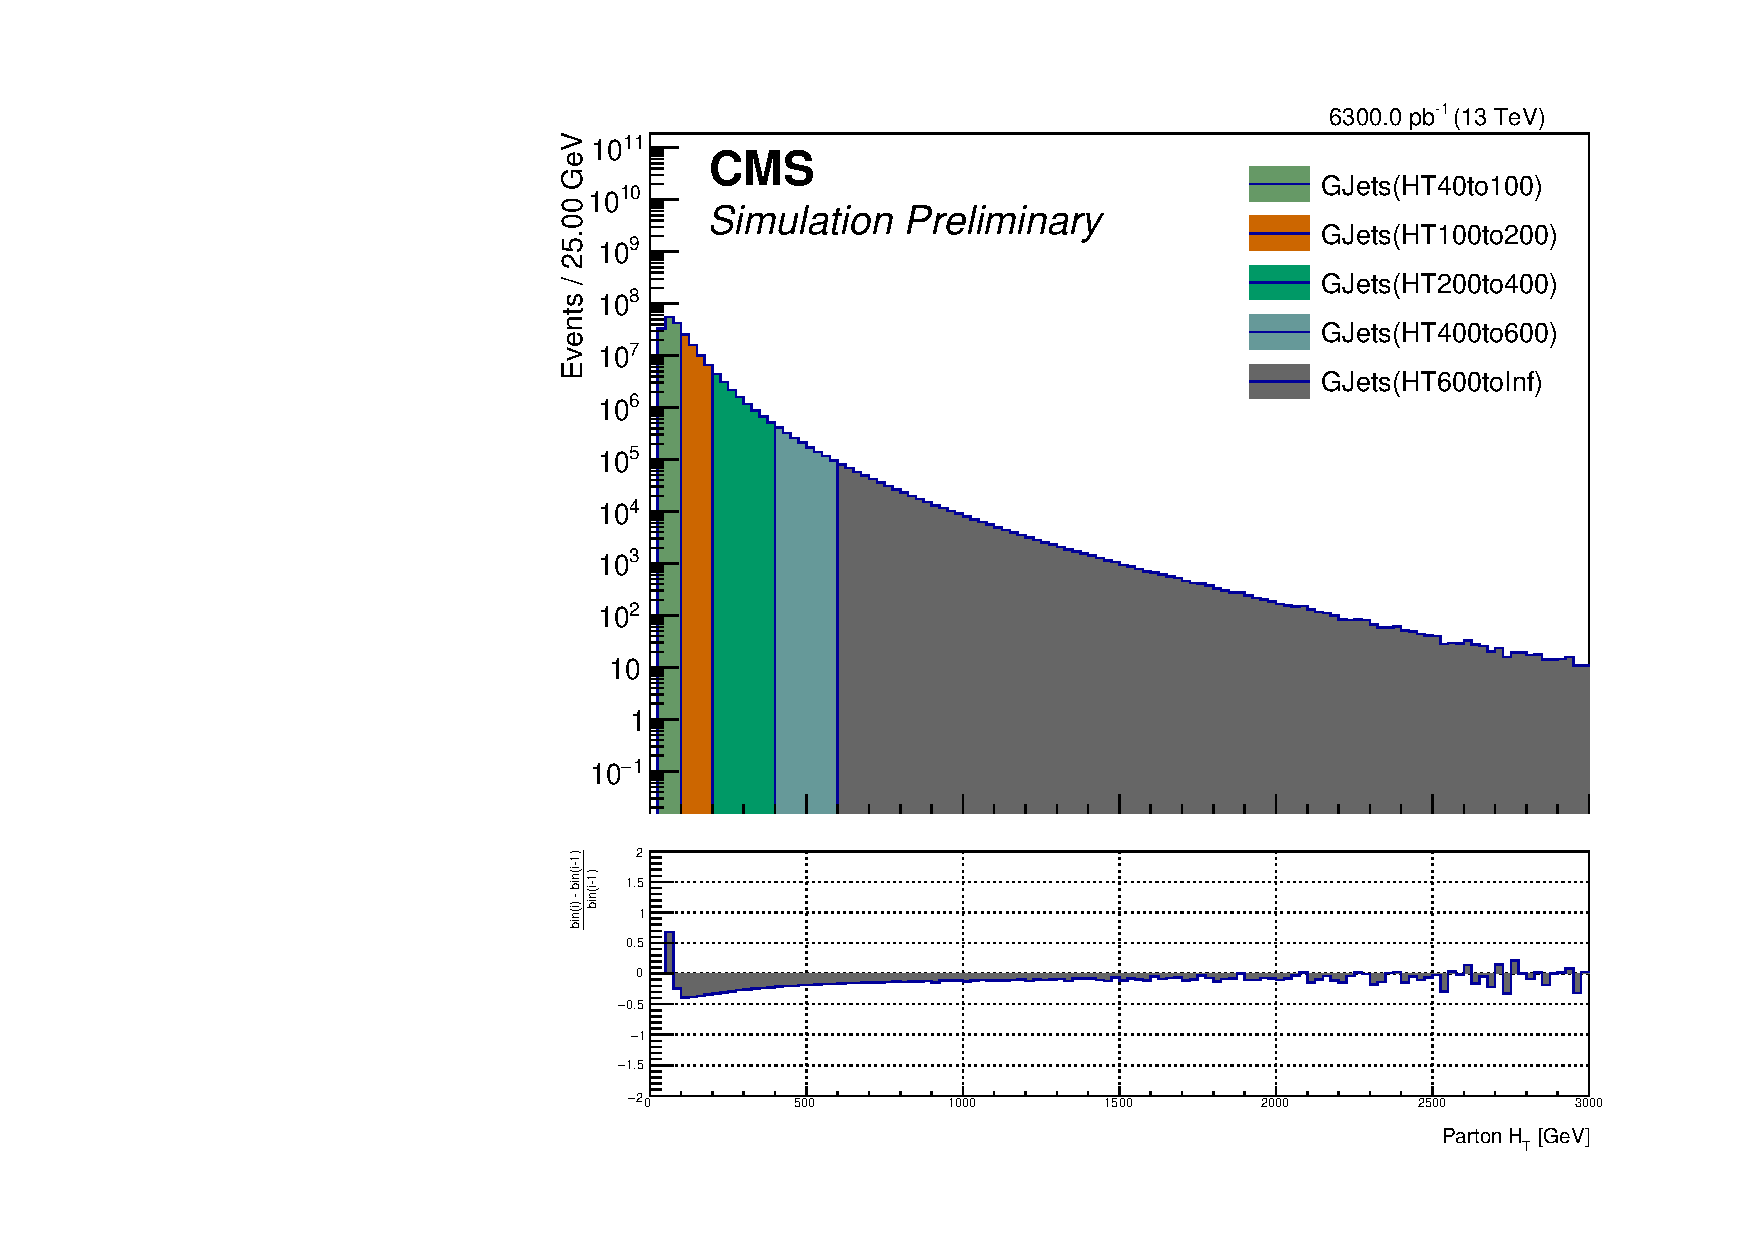
\includegraphics[width=0.35\textwidth]{figures/binnedMCsamples/GJets_HT.pdf}} ~
    \subfigure[\ttbar\ + jets]{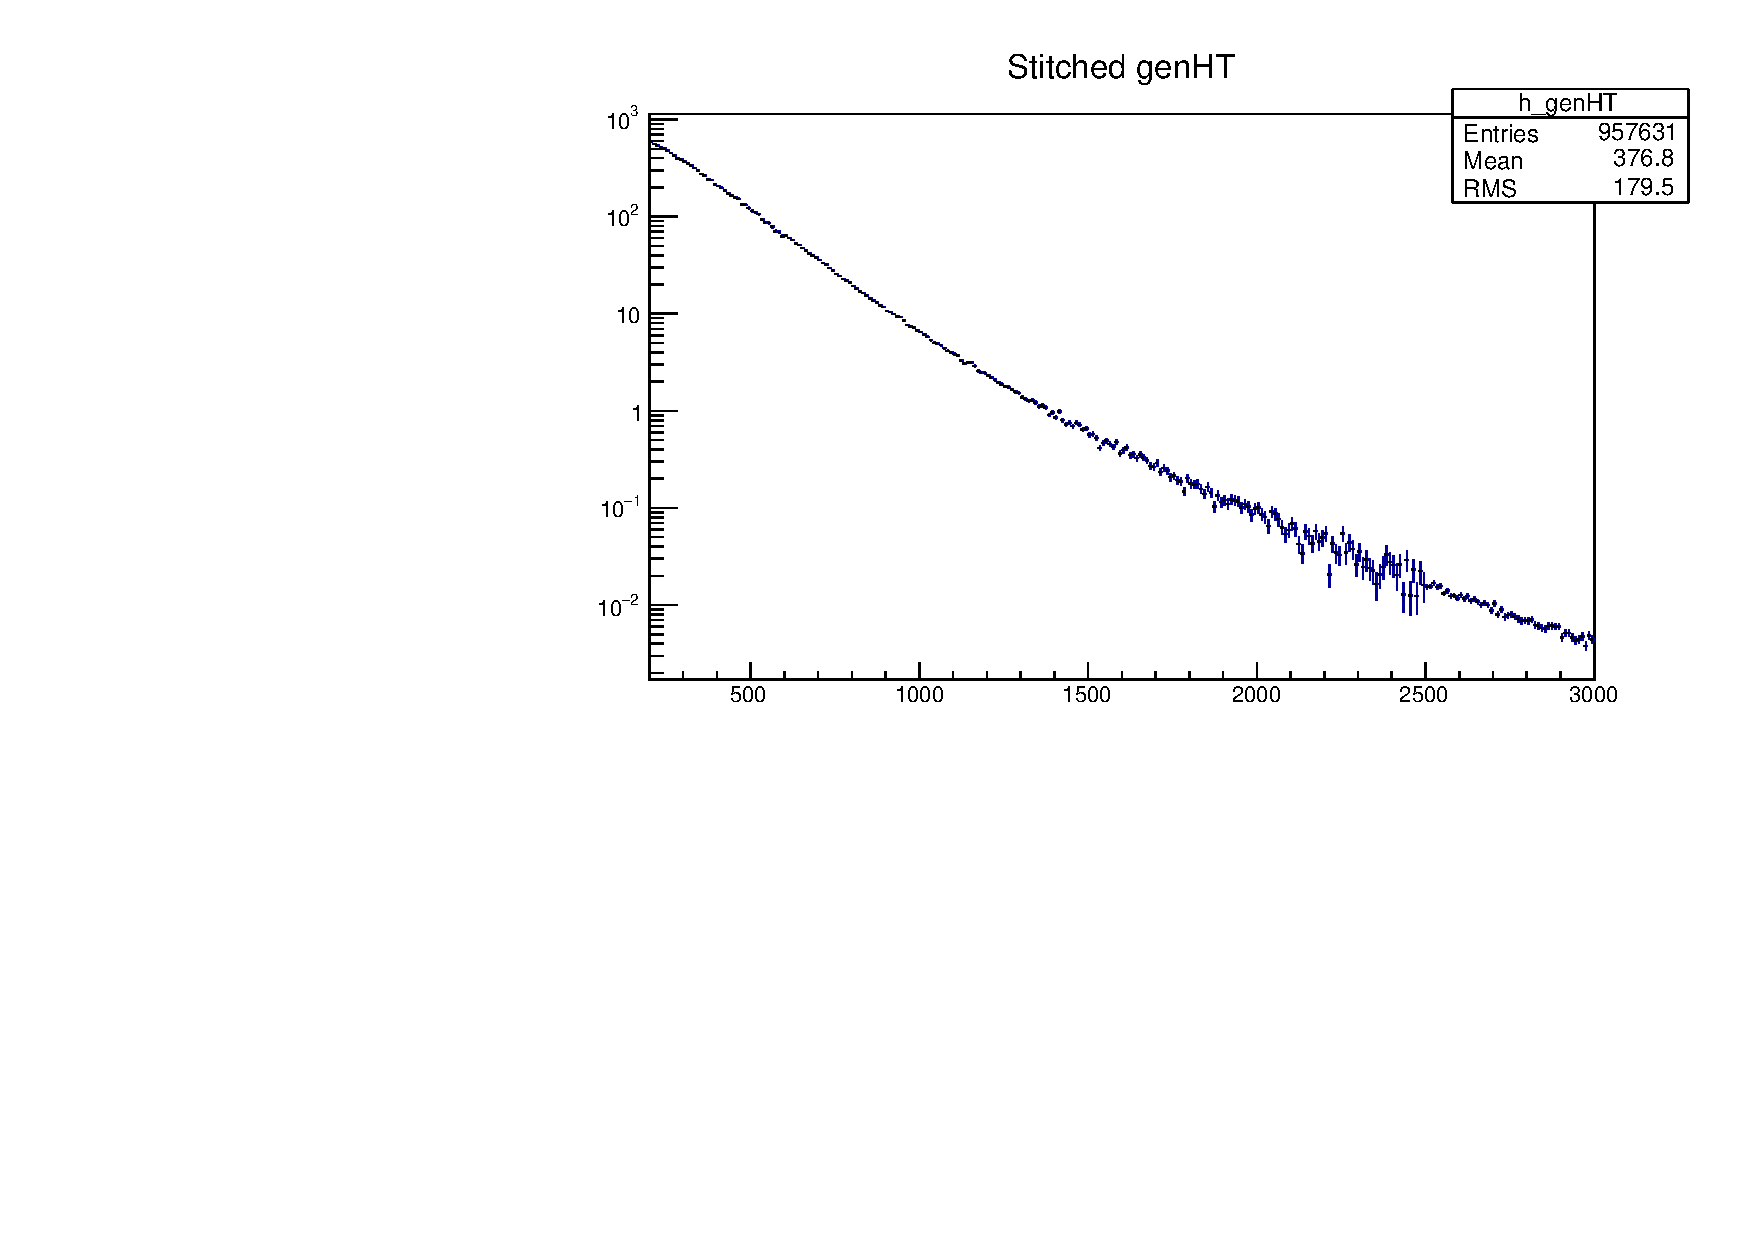
\includegraphics[width=0.35\textwidth]{figures/binnedMCsamples/TTbar.pdf}} 
    \caption{Generator-level parton \scalht distributions for SM
      process, $Z\rightarrow \nu\nu$ + jets, W + jets, DY + jets, QCD,
      \gj, and \ttbar\ + jets (subsamples not shown). }
    \label{fig:Lhe_Ht}
  \end{center}
\end{figure}

\begin{table}[h!]
  \centering
  \topcaption{Simulated event samples of signal processes used
    by this analysis. Symbols used as shorthand are defined at the
    bottom of the table. 
  }
  \footnotesize
  \begin{longtable}{| c | c | c | c | c | c | c | c | c  | }
\caption{Summary of yields of each SM process} \label{tab:table} \\    \hline 
$n_{j}$~$n_{b}$~$H_{T}$ & $t\bar{t}$ & $W+jets$ & $Z \rightarrow \nu\nu$ & $DY+jets$ & $Single Top$ & $DiBoson$ & $Multijet$ & Total Yield\\ \hline 
eq2j eq0b 200 & 103.49 & 1026.57 & 1148.86 & 18.24 & 15.98 & 72.15 & 0.00 & 2385.28\\ \hline 
eq2j eq0b 250 & 74.63 & 1050.96 & 1312.16 & 16.09 & 15.33 & 74.25 & 10.11 & 2553.53\\ \hline 
eq2j eq0b 300 & 32.27 & 664.60 & 941.01 & 9.13 & 6.52 & 42.69 & 2.85 & 1699.07\\ \hline 
eq2j eq0b 350 & 12.65 & 395.06 & 569.00 & 5.50 & 1.62 & 17.06 & 1.33 & 1002.24\\ \hline 
eq2j eq0b 400 & 7.22 & 316.98 & 551.29 & 3.96 & 2.22 & 14.28 & 1.51 & 897.46\\ \hline 
eq2j eq0b 500 & 1.33 & 102.97 & 190.11 & 0.79 & 0.01 & 2.12 & 0.00 & 297.31\\ \hline 
eq2j eq0b 600 & 0.47 & 50.93 & 111.12 & 0.29 & 0.54 & 2.69 & 0.00 & 166.04\\ \hline 
eq2j eq0b 800 & 0.52 & 86.65 & 146.22 & 0.39 & 0.00 & 3.16 & 0.00 & 236.94\\ \hline 
eq3j eq1b 200 & 0.57 & 0.00 & 0.32 & 0.00 & 0.00 & 0.00 & 0.00 & 0.89\\ \hline 
eq3j eq1b 250 & 64.13 & 17.16 & 27.10 & 0.54 & 5.36 & 1.22 & 0.00 & 115.51\\ \hline 
eq3j eq1b 300 & 122.13 & 56.55 & 74.29 & 1.00 & 13.99 & 2.69 & 0.00 & 270.64\\ \hline 
eq3j eq1b 350 & 94.34 & 52.60 & 82.06 & 0.85 & 13.66 & 5.30 & 6.22 & 255.03\\ \hline 
eq3j eq1b 400 & 71.61 & 66.57 & 99.75 & 0.82 & 15.02 & 3.06 & 0.43 & 257.26\\ \hline 
eq3j eq1b 500 & 11.23 & 18.94 & 42.91 & 0.24 & 1.88 & 1.61 & 0.00 & 76.82\\ \hline 
eq3j eq1b 600 & 2.92 & 10.44 & 26.73 & 0.12 & 0.66 & 1.20 & 0.00 & 42.06\\ \hline 
eq3j eq1b 800 & 1.93 & 11.73 & 29.27 & 0.07 & 0.54 & 1.37 & 0.00 & 44.92\\ \hline 
eq4j eq2b 200 & 0.00 & 0.00 & 0.00 & 0.00 & 0.00 & 0.00 & 0.00 & 0.00\\ \hline 
eq4j eq2b 250 & 0.20 & 0.00 & 0.02 & 0.00 & 0.00 & 0.00 & 0.00 & 0.22\\ \hline 
eq4j eq2b 300 & 18.30 & 0.75 & 1.98 & 0.01 & 1.38 & 0.00 & 0.00 & 22.42\\ \hline 
eq4j eq2b 350 & 56.98 & 4.03 & 6.78 & 0.08 & 3.56 & 0.00 & 0.00 & 71.43\\ \hline 
eq4j eq2b 400 & 86.02 & 6.97 & 12.42 & 0.11 & 4.54 & 0.60 & 0.00 & 110.66\\ \hline 
eq4j eq2b 500 & 21.45 & 2.68 & 7.27 & 0.05 & 2.76 & 0.25 & 0.00 & 34.46\\ \hline 
eq4j eq2b 600 & 5.24 & 2.02 & 4.38 & 0.02 & 1.26 & 0.05 & 0.00 & 12.98\\ \hline 
eq4j eq2b 800 & 2.66 & 0.00 & 3.79 & 0.02 & 0.58 & 0.00 & 0.00 & 7.06\\ \hline 
ge5j eq0b 200 & 0.00 & 0.00 & 0.00 & 0.00 & 0.00 & 0.00 & 0.00 & 0.00\\ \hline 
ge5j eq0b 250 & 0.00 & 0.00 & 0.00 & 0.00 & 0.00 & 0.00 & 0.00 & 0.00\\ \hline 
ge5j eq0b 300 & 0.03 & 0.00 & 0.05 & 0.00 & 0.00 & 0.00 & 0.00 & 0.07\\ \hline 
ge5j eq0b 350 & 6.96 & 8.88 & 7.98 & 0.26 & 0.00 & 0.39 & 0.02 & 24.49\\ \hline 
ge5j eq0b 400 & 57.77 & 102.86 & 111.49 & 1.65 & 3.35 & 4.48 & 0.00 & 281.60\\ \hline 
ge5j eq0b 500 & 41.04 & 96.56 & 124.97 & 1.30 & 1.62 & 1.67 & 8.83 & 275.99\\ \hline 
ge5j eq0b 600 & 26.59 & 91.74 & 128.08 & 0.96 & 2.62 & 3.95 & 1.72 & 255.67\\ \hline 
ge5j eq0b 800 & 16.75 & 67.00 & 130.94 & 0.76 & 1.84 & 2.45 & 6.82 & 226.57\\ \hline 
    \hline 
    \hline 
\end{longtable}

  \label{tab:datasets_signal}
\end{table}

%%____________________________________________________________________________||
